\section{EXPERIMENTS}
\label{sec:experiments}

The created architecture was tested in two environments: a simulation and a real.
The real agents are as shown the figure \ref{fig:agents}.
The primary objective was to prove that the connection and exchange of information occurs between the agents, in such way that each agent know about the others and can perform actions based on this knowledge.

To proof the \emph{Droid} package, two simulation tests was performed: (i) the following mode, where a agent must follow and maintain a certain distance from another target agent, and (ii) the obstacle mode, where a terrestrial agent can ask for help to a aerial agent if it detects that is not possible to complete your mission.

\begin{figure}[ht!]
  \centering
  \begin{subfigure}[b]{0.8\columnwidth}
    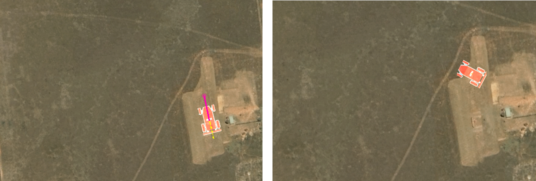
\includegraphics[width=\textwidth]{img/follow1.png}
  \end{subfigure}
  \begin{subfigure}[b]{0.8\columnwidth}
    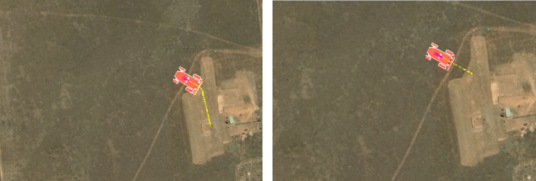
\includegraphics[width=\textwidth]{img/follow2.png}
  \end{subfigure}
  \begin{subfigure}[b]{0.8\columnwidth}
    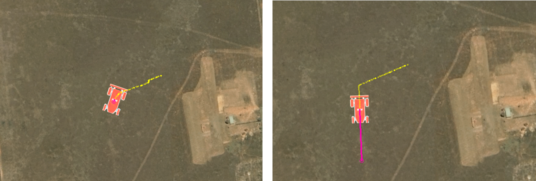
\includegraphics[width=\textwidth]{img/follow3.png}
  \end{subfigure}
  \begin{subfigure}[b]{0.8\columnwidth}
    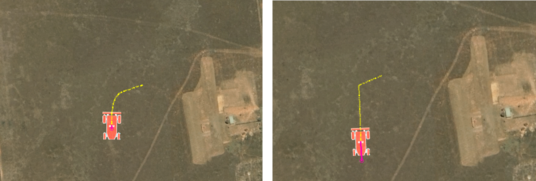
\includegraphics[width=\textwidth]{img/follow4.png}
  \end{subfigure}
  \begin{subfigure}[b]{0.8\columnwidth}
    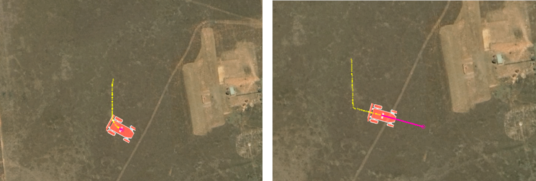
\includegraphics[width=\textwidth]{img/follow5.png}
  \end{subfigure}
  \begin{subfigure}[b]{0.8\columnwidth}
    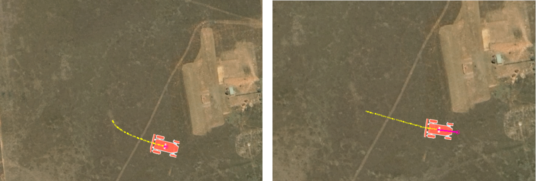
\includegraphics[width=\textwidth]{img/follow6.png}
  \end{subfigure}
  \begin{subfigure}[b]{0.8\columnwidth}
    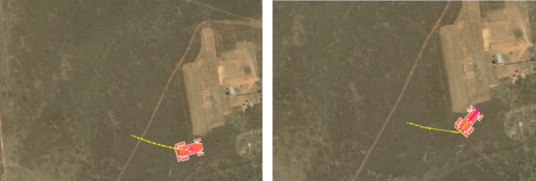
\includegraphics[width=\textwidth]{img/follow7.png}
  \end{subfigure}

  \caption{Two rovers in simulation, the right rover executes his mission while the left rover follows it.}
  \label{fig:simulation}
\end{figure}

\begin{figure*}
  \centering
  \begin{subfigure}[b]{0.9\columnwidth}
    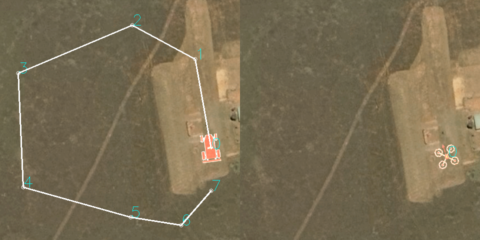
\includegraphics[width=\textwidth]{img/mission1.png}
    \caption{Mission start.}
  \end{subfigure}
  \begin{subfigure}[b]{0.9\columnwidth}
    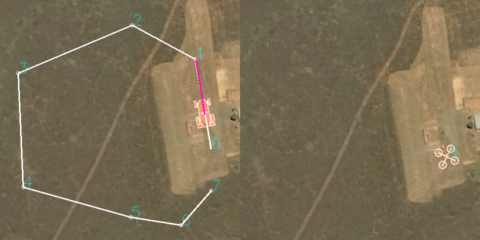
\includegraphics[width=\textwidth]{img/mission2.png}
    \caption{Go to waypoint 1.}
  \end{subfigure}
  \begin{subfigure}[b]{0.9\columnwidth}
    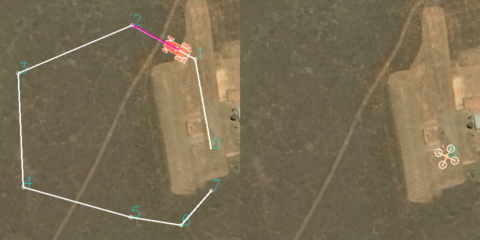
\includegraphics[width=\textwidth]{img/mission3.png}
    \caption{Go to waypoint 2.}
  \end{subfigure}
  \begin{subfigure}[b]{0.9\columnwidth}
    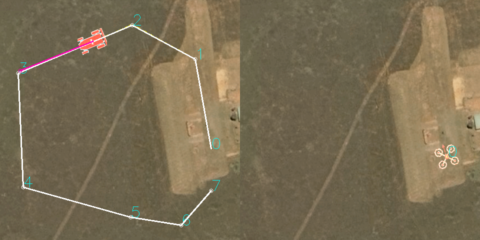
\includegraphics[width=\textwidth]{img/mission4.png}
    \caption{Go to waypoint 3.}
  \end{subfigure}
  \begin{subfigure}[b]{0.9\columnwidth}
    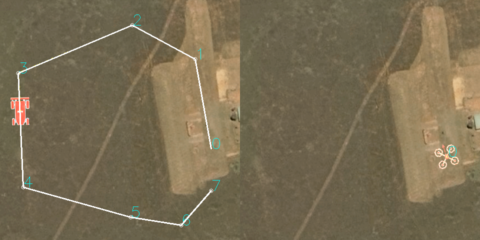
\includegraphics[width=\textwidth]{img/mission5.png}
    \caption{Go to waypoint 4, but found a obstacle.}
  \end{subfigure}
  \begin{subfigure}[b]{0.9\columnwidth}
    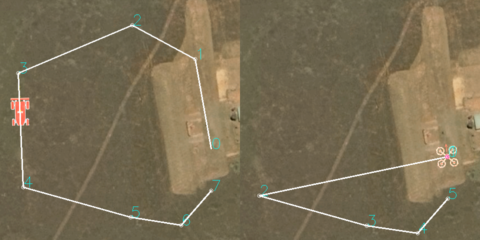
\includegraphics[width=\textwidth]{img/mission6.png}
    \caption{Request help and send the remainder mission.}
  \end{subfigure}
  \begin{subfigure}[b]{0.9\columnwidth}
    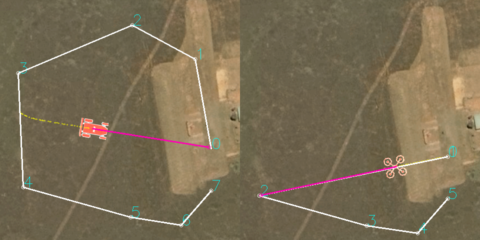
\includegraphics[width=\textwidth]{img/mission7.png}
    \caption{Return to home while other agent take the mission.}
  \end{subfigure}
  \begin{subfigure}[b]{0.9\columnwidth}
    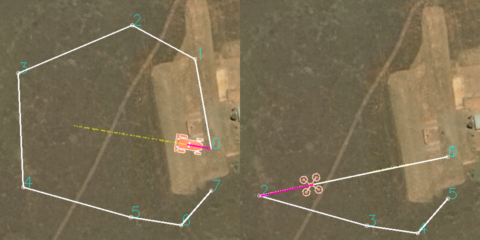
\includegraphics[width=\textwidth]{img/mission8.png}
    \caption{Reach home and the helper agent start the mission.}
  \end{subfigure}
  \begin{subfigure}[b]{0.9\columnwidth}
    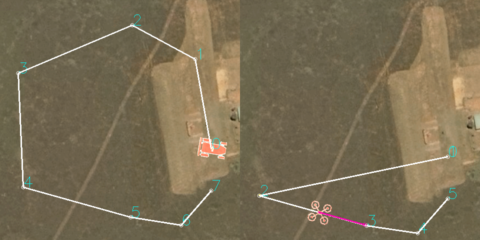
\includegraphics[width=\textwidth]{img/mission9.png}
    \caption{The agent continue the mission.}
  \end{subfigure}
  \begin{subfigure}[b]{0.9\columnwidth}
    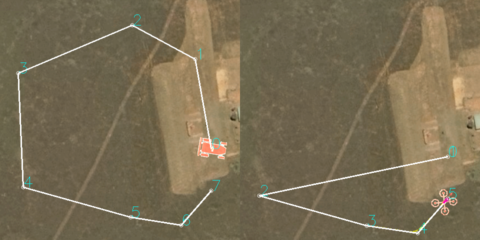
\includegraphics[width=\textwidth]{img/mission10.png}
    \caption{Mission complete by the other agent.}
  \end{subfigure}

  \caption{Mission execution by the rover agent, that founds a obstacles and ask for help to another agent.}
  \label{fig:simulation_mission}
\end{figure*}

The following mode test is demonstrated in the figure \ref{fig:simulation} (simulation environment) and \ref{fig:real} (real experiment), where one robot is executing a determined mission, but sharing its current position the other agents in the team, and another robot use this information to follow that agent, but keeping a configurable safety distance.

% The figure \ref{fig:simulation} show the two agents in the simulation representation.
% They have similar capabilities compared to the real robots, but with a best control and maneuverability, considering that a simulation will not is equal to a real environment.

\begin{figure}[ht!]
  \centering
  \begin{subfigure}[b]{0.8\columnwidth}
    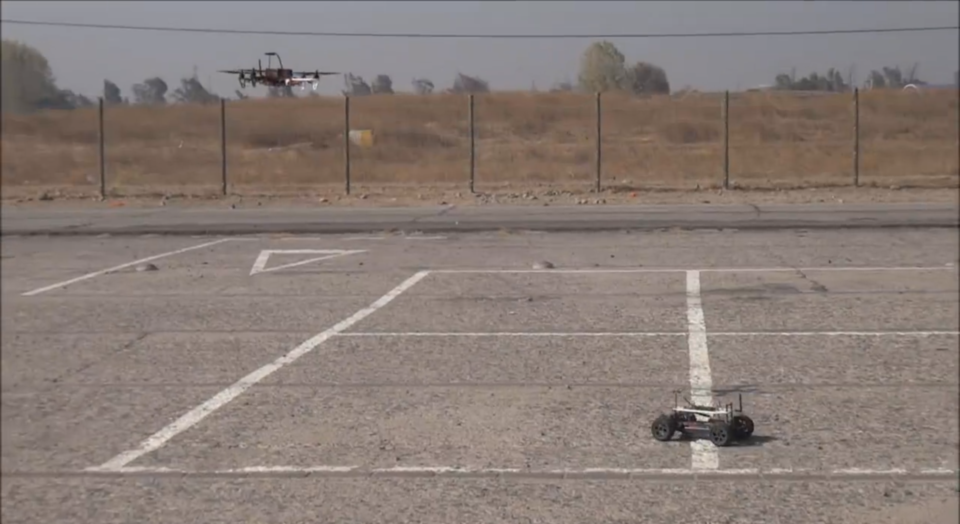
\includegraphics[width=\textwidth]{img/follow_real1.png}
  \end{subfigure}
  \begin{subfigure}[b]{0.8\columnwidth}
    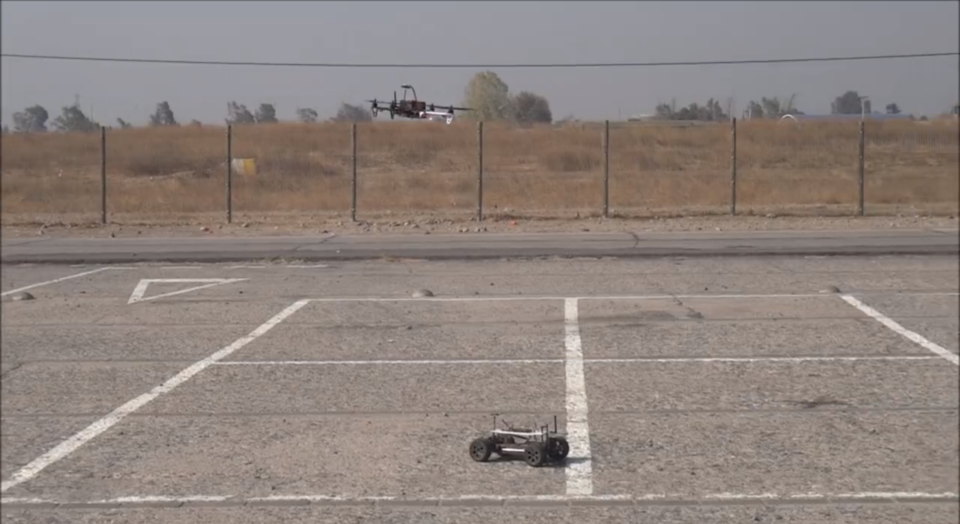
\includegraphics[width=\textwidth]{img/follow_real2.png}
  \end{subfigure}
  \begin{subfigure}[b]{0.8\columnwidth}
    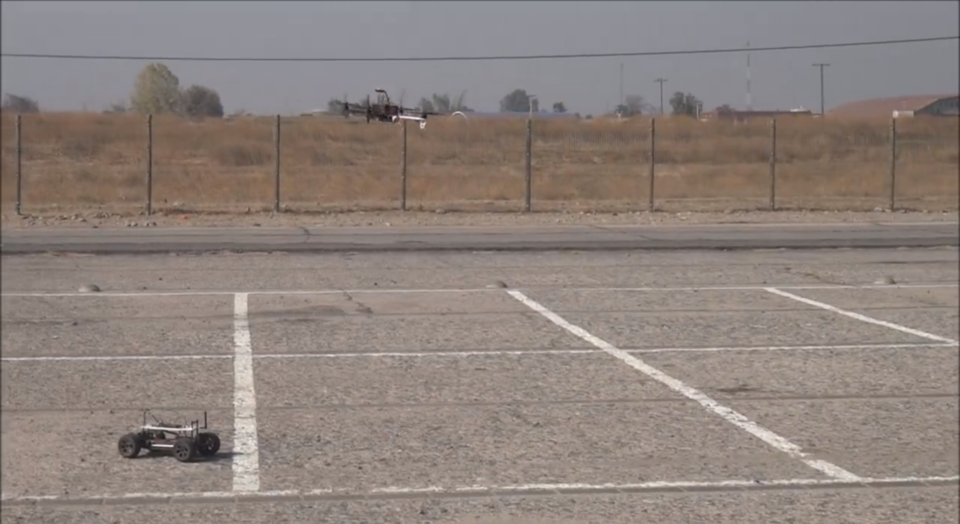
\includegraphics[width=\textwidth]{img/follow_real3.png}
  \end{subfigure}
  \begin{subfigure}[b]{0.8\columnwidth}
    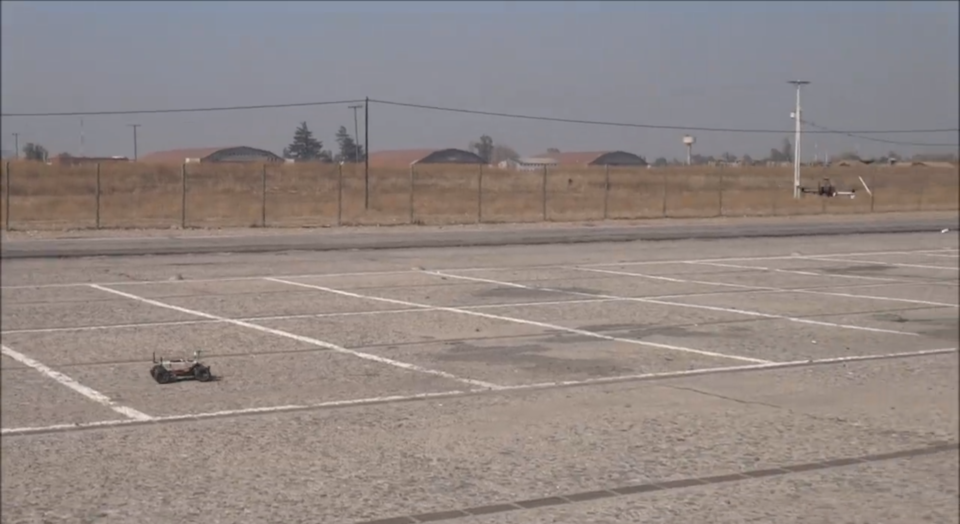
\includegraphics[width=\textwidth]{img/follow_real4.png}
  \end{subfigure}

  \caption{Real experiment showing the follow mode using a rover vehicle and a quadrotor drone.}
  \label{fig:real}
\end{figure}

The test shown in the figure \ref{fig:simulation_mission} demonstrate the behavior where a agent founds a obstacle which prevents your mission conclusion, and then ask to another agent to finish it, sending the remaining mission and returning the home.

These tests were developed to demonstrate that the architecture extension works to communicate and take decisions based on data sent by the agents, performing actions using the resources available for the team of robots.

% The first test applied was to just make one agent follow another while
